% =============================================================================
% 05_diagnostics.tex  --  Chapter 5, Diagnostics: how each failure was isolated
% Plan: docs/thesis/REWRITE_PLAN.md sections 1.7, 2 ("5 Diagnostics"), 4 (T8, T9, T10, T14, T18), 5 (rules).
% Numbers: numbers_diagnostics.tex (macros \Diag...), loaded by numbers.tex; loaded here only when compiled alone.
% Tables owned here: tables/T08_depth_runs, T09_neck, T10_fingers, T14_pilot_noise, T18_shape_head.
% Figures: F6 (exists), F23 and F24 (pending cluster files) as \IfFileExists placeholders; F15 (depth scatter) and
% F13 (real photos) are owned by other files and only referenced.
% Labels used from other chapters: ch:method, ch:results, tab:relhuman (T12), fig:depth-scatter (F15),
% fig:final-real-photos (F13), fig:neck-3dpw (F9).
% =============================================================================

\ifdefined\DiagNumbersLoaded\else% =============================================================================
% numbers_diagnostics.tex -- numbers of Chapter 5 (Diagnostics), one macro each, prefix \Diag.
% Convention: numbers.tex. Source on every line. Source key as in REWRITE_PLAN.md:
%   H x.y = docs/handover.md section x.y; H 0b = "Numbers at a glance"; H 1 = "Project in brief";
%   F = docs/diagnostics_findings.md (section name in quotes); D = docs/deck_explained_2026-10-19.md;
%   CE = task note children_evidence.md (scratchpad tasks/); NNNNNNN:LL = line of that Slurm log (via the handover).
% Setting unless noted: Base (v5 epoch 99), V1, 100-image AnnyOne holdout (579,860-579,959), matched people.
% Signed values carry \ensuremath{-...}; use \Diag...{} before a following word.
% =============================================================================
\newcommand{\DiagNumbersLoaded}{}

% ---------------------------------------------------------------- sets
\newcommand{\DiagHoldoutImages}{100}          % H 1 "Data"
\newcommand{\DiagHoldoutPeople}{222}          % F "The depth defect" (E1, 222 people kept)

% ---------------------------------------------------------------- 5.1 visible failures / old child evidence
\newcommand{\DiagSmallPeopleAgeLow}{0.57}     % H 6 "Children" (old claim "age 0.57-0.67"); F "Children" (E4 0.56-0.66 range)
\newcommand{\DiagSmallPeopleAgeHigh}{0.67}    % H 6 "Children"
\newcommand{\DiagSmallPeopleHeightLow}{0.47}  % height phenotype, 3569949/3572419/3572420 lines 7-71 (H 3.4; CE)
\newcommand{\DiagSmallPeopleHeightHigh}{0.56} % same
\newcommand{\DiagBoyAge}{0.60}                % the boy in 360_F_392252267...jpg, H 3.4 "real-photo measurement, corrected"
\newcommand{\DiagBoyHeight}{0.48}             % same

% ---------------------------------------------------------------- 5.2 six checks
\newcommand{\DiagGTInsideImage}{84.5}         % percent, F "Check 1"
\newcommand{\DiagGTInsideBox}{84.9}           % percent, F "Check 1"
\newcommand{\DiagAgeSweepLow}{0.53}           % m, skeletal height at age 0 (0.528), F "Checks 2+3" (= \DataSweepHeightAgeZero)
\newcommand{\DiagAgeSweepHigh}{1.55}          % m, at age 0.8 (1.553), F "Checks 2+3"; deck D slide 11 says 1.54 m "age 0 to 1"
\newcommand{\DiagHeadRatioLow}{0.200}         % head/height at age 0, F "Checks 2+3"
\newcommand{\DiagHeadRatioHigh}{0.106}        % head/height at age 0.8, F "Checks 2+3"
\newcommand{\DiagPerturbations}{16}           % single-joint perturbations, all PASS, F "Checks 2+3"
\newcommand{\DiagHelperBones}{88}             % F "Check 4"; H 1
\newcommand{\DiagActiveBones}{75}             % F "Check 4"; H 1
\newcommand{\DiagShapeOutputs}{11}            % H 1 "What is not the cause"; D slide 11
\newcommand{\DiagGradRoot}{598}               % per-bone |grad|, F "Check 4"
\newcommand{\DiagGradFingers}{4.7}            % per-bone |grad|, F "Check 4"
\newcommand{\DiagLossShareShape}{25.7}        % percent of loss at epoch 99, F "Check 4"
\newcommand{\DiagLossShareTransl}{1.9}        % percent, F "Check 4"
\newcommand{\DiagLossShareDist}{0.6}          % percent, F "Check 4"
\newcommand{\DiagLossShareDepthTerms}{2.5}    % percent, transl + dist, F "The depth defect"
\newcommand{\DiagNeckLengthPct}{99.3}         % predicted neck length / GT, percent, F "Neck"
\newcommand{\DiagChildSwapBefore}{47.8}       % mm PVE, 10 manifest children, F "Children"
\newcommand{\DiagChildSwapAfter}{41.6}        % mm PVE with GT shape, F "Children" (gain 6.2 mm)
\newcommand{\DiagOverfitTrainBefore}{80.7}    % mm, V0, F "Check 6"
\newcommand{\DiagOverfitTrainAfter}{51.8}     % mm, F "Check 6"
\newcommand{\DiagOverfitTrainDrop}{36}        % percent, F "Check 6"
\newcommand{\DiagOverfitHoldBefore}{87.6}     % mm, F "Check 6"
\newcommand{\DiagOverfitHoldAfter}{127.2}     % mm, F "Check 6"
\newcommand{\DiagOverfitHoldRise}{45}         % percent, F "Check 6"
\newcommand{\DiagOverfitRotFirst}{44.6}       % rotmat term, mean of first 5 logged epochs, F "Check 6"; D slide 11
\newcommand{\DiagOverfitRotLast}{40.8}        % mean of last 5, F "Check 6"
\newcommand{\DiagOverfitTranslFirst}{1.67}    % transl term, first 5, F "Check 6"; H 1 "What is not the cause"
\newcommand{\DiagOverfitTranslLast}{1.89}     % last 5, same
\newcommand{\DiagOverfitTwoDFirst}{58}        % j2d term, first 5, same
\newcommand{\DiagOverfitTwoDLast}{75}         % last 5, same
\newcommand{\DiagOverfitTranslHalfA}{2.10}    % first-half average, H 1 "What is not the cause" [Guessing there]
\newcommand{\DiagOverfitTranslHalfB}{1.96}    % second-half average, same
\newcommand{\DiagOverfitTwoDHalfA}{69}        % same
\newcommand{\DiagOverfitTwoDHalfB}{63}        % same

% ---------------------------------------------------------------- 5.3 depth (placement table, T8)
\newcommand{\DiagDepthTrueMean}{1.92}         % m, F "The depth defect" table
\newcommand{\DiagDepthTrueSd}{0.49}           % m, same
\newcommand{\DiagDepthPredMean}{3.00}         % m, same
\newcommand{\DiagDepthPredSd}{0.32}           % m, same
\newcommand{\DiagDepthSlopeBase}{0.33}        % 3571596:64 (H 3.1); F
\newcommand{\DiagDepthInterceptBase}{2.36}    % m, same
\newcommand{\DiagDepthFartherPct}{100}        % percent of people predicted farther, F "The depth defect"
\newcommand{\DiagDepthCorrError}{\ensuremath{-0.76}} % corr(GT depth, depth error), F "The depth defect"
\newcommand{\DiagSkelHeightTrue}{1.409}       % m, F "The depth defect"
\newcommand{\DiagSkelHeightPred}{1.405}       % m, same
\newcommand{\DiagSkelHeightCorr}{0.89}        % r, same
\newcommand{\DiagSizeBase}{0.63}              % trace size ratio, H 3.1 (not the findings' 0.65/0.67, H 6)
\newcommand{\DiagRootErrBase}{1.21}           % m, absolute root error, 3571596:55 (H 3.1)
\newcommand{\DiagHeadPxBase}{64.5}            % px mean, F "Baseline numbers"; H 3.1
\newcommand{\DiagHeadPxBaseMedian}{46}        % px median, F "Baseline numbers"
\newcommand{\DiagPelvisPxBase}{23.4}          % px mean, F "Baseline numbers"; H 3.1
\newcommand{\DiagPelvisPxBaseMedian}{14}      % px median, F "Baseline numbers"
\newcommand{\DiagCorrPVEDepth}{\ensuremath{-0.03}} % corr(PVE, depth error), F "The depth defect"
\newcommand{\DiagOffsetMin}{\ensuremath{-2}}  % cells, --debug_anchor print, 3571599:9-14 (H 3.1)
\newcommand{\DiagOffsetMax}{\ensuremath{-19}} % cells, same
\newcommand{\DiagRootErrFixLow}{0.53}         % m, 2-ep x20, 3572483 (H 3.1)
\newcommand{\DiagRootErrFixHigh}{0.73}        % m, 10-ep x1, 3571933 (H 3.1); final 0.728
\newcommand{\DiagRootErrCtrlLow}{1.11}        % m, 2-ep control, 3571599 (H 3.1)
\newcommand{\DiagRootErrCtrlHigh}{1.44}       % m, 10-ep control, 3571934 (H 3.1)
\newcommand{\DiagSizeCtrlLow}{0.59}           % H 3.1 / H 0b
\newcommand{\DiagSizeCtrlHigh}{0.66}          % H 3.1
\newcommand{\DiagSizeFixLow}{0.78}            % H 3.1
\newcommand{\DiagSizeFixHigh}{0.87}           % H 3.1
\newcommand{\DiagFinalRootErr}{0.73}          % m (728 mm), 3611336:175 (H 3.1)
\newcommand{\DiagControlRootErr}{1.40}        % m (1402 mm), 3611339:166 (H 3.1)
\newcommand{\DiagFinalSize}{0.78}             % 3611336:184 (H 3.1)
\newcommand{\DiagControlSize}{0.59}           % 3611339:175 (H 3.1)
\newcommand{\DiagFinalSlope}{0.42}            % 3611336:184 (H 3.1)
\newcommand{\DiagControlSlope}{0.28}          % 3611339:175 (H 3.1)
\newcommand{\DiagOldRootErrA}{1.39}           % m, Base+3DPW(old labels) e62, 3571963 (H 3.1)
\newcommand{\DiagOldRootErrB}{1.49}           % m, fresh-head run (v10 e290), 3571794 (H 3.1)
\newcommand{\DiagSlopeSwitch}{0.30}           % 2-ep and 10-ep fix x1, H 3.1
\newcommand{\DiagSlopeStrongLow}{0.38}        % 10-ep x5, H 3.1
\newcommand{\DiagSlopeStrongHigh}{0.44}       % 2-ep x5, H 3.1
\newcommand{\DiagFixCostPVELow}{2.6}          % mm vs own control, H 3.1 (+2.58)
\newcommand{\DiagFixCostPVEHigh}{4.9}         % mm, H 3.1 (+4.93)
\newcommand{\DiagFixCostRecallLow}{1.6}       % points, H 3.1; H 0b
\newcommand{\DiagFixCostRecallHigh}{2.4}      % points, same

% ---------------------------------------------------------------- 5.4 neck (dump, T9)
\newcommand{\DiagDumpNeckOne}{5.3}            % deg, 3573518:12 (H 3.2)
\newcommand{\DiagDumpNeckTwo}{175.6}          % deg, 3573518:13
\newcommand{\DiagDumpNeckTwoTwist}{175.7}     % deg, 3573518:13
\newcommand{\DiagDumpNeckTwoSwing}{3.3}       % deg, 3573518:13
\newcommand{\DiagDumpNeckThree}{5.7}          % deg local, 3573518:14
\newcommand{\DiagDumpNeckThreeGlobal}{173.3}  % deg global, 3573518:14
\newcommand{\DiagDumpHead}{177.9}             % deg, 3573518:15
\newcommand{\DiagDumpHeadGlobal}{12.0}        % deg global, 3573518:15
\newcommand{\DiagDumpJaw}{2.2}                % deg, 3573518:16
\newcommand{\DiagNeckGirthBase}{0.46}         % 0.461, 3573518:69; 3579014:107
\newcommand{\DiagNeckSkinBase}{27.3}          % mm PVE_neck, 3573518:69
\newcommand{\DiagNeckTwoRangeLow}{175.0}      % deg, all 8 v5-line checkpoints, H 3.2
\newcommand{\DiagNeckTwoRangeHigh}{176.0}     % deg, same
\newcommand{\DiagGirthRangeLow}{0.46}         % H 3.2 (long_pc_dist5 0.457, 3573518:357-360)
\newcommand{\DiagGirthRangeHigh}{0.47}        % H 3.2 (exp5 geodesic 0.468, 3573521:61)
\newcommand{\DiagFreshGirth}{1.00}            % v10, 3573518:189 (H 3.2)
\newcommand{\DiagFreshNeckSkin}{10.3}         % mm, v10, 3573518:191
\newcommand{\DiagNeckTwoBase}{175.6}          % deg, 3579014:101
\newcommand{\DiagGeodesicNeckTwo}{175.0}      % deg, exp5 geodesic, 3573521:89-91 (H 3.2)
\newcommand{\DiagGeodesicHead}{177.1}         % deg, same
\newcommand{\DiagCorrNeckTwo}{178.8}          % deg, correction constant, 3579014:12, :37
\newcommand{\DiagCorrHead}{179.2}             % deg, same
\newcommand{\DiagCorrMetacarpal}{179.8}       % deg, same
\newcommand{\DiagCorrFinger}{179.7}           % deg, same
\newcommand{\DiagNeckTwoNoTrain}{4.5}         % deg, 3579014:101
\newcommand{\DiagGirthNoTrain}{1.004}         % 3579014:107
\newcommand{\DiagNeckSkinNoTrain}{10.8}       % mm, 3579014:108
\newcommand{\DiagHeadDirBase}{12.0}           % deg global head, 3579014:113
\newcommand{\DiagHeadDirNoTrain}{19.1}        % deg, 3579014:113; verdict :120
\newcommand{\DiagHeadDirFineTune}{14.4}       % deg, 3579014:113
\newcommand{\DiagHeadDirCtrlTwo}{13.8}        % deg, exp5 L1 control, 3579014:113
\newcommand{\DiagPVEBase}{70.5}               % mm, 3570222:40; 3579014:109
\newcommand{\DiagPVENoTrain}{71.3}            % mm, 3579014:109
\newcommand{\DiagPVEFineTune}{68.8}           % mm, 3579014:109
\newcommand{\DiagPVECtrlTwo}{76.9}            % mm, 3579014:109; 3573521:98
\newcommand{\DiagFinalNeckTwo}{4.8}           % deg, 3611336:202,206
\newcommand{\DiagFinalHeadBone}{8.9}          % deg, 3611336:203,207
\newcommand{\DiagFinalGirth}{0.996}           % 3611336:198
\newcommand{\DiagFinalNeckSkin}{11.0}         % mm, 3611336:199
\newcommand{\DiagFinalHeadDir}{13.1}          % deg, 3611336:200
\newcommand{\DiagControlHeadDir}{13.0}        % deg, 3611339:191

% ---------------------------------------------------------------- 5.5 fingers (T10)
\newcommand{\DiagFingersBase}{17.3}           % deg, 3571960:290 (H 3.3)
\newcommand{\DiagFingersRest}{15.1}           % deg, --relax_hands, 3571960:290
\newcommand{\DiagHandTokens}{2.25}            % tokens, median, 3571960:287
\newcommand{\DiagHandUnderTwo}{41}            % percent under 2 tokens, 3571960:287
\newcommand{\DiagFingersZoom}{17.2}           % deg, test-time crop, 3571960:299
\newcommand{\DiagZoomPVE}{124.8}              % mm, body PVE on crops, 3571960:294
\newcommand{\DiagFingersRegion}{17.5}         % deg, region-normalised loss, 3571959:316
\newcommand{\DiagFingersRegionCtrl}{17.4}     % deg, its control, 3571960:314
\newcommand{\DiagFingersFixNoTrain}{8.2}      % deg, 3579014:114
\newcommand{\DiagFingersFixFT}{8.3}           % deg, 3579014:114
\newcommand{\DiagFingersFinal}{8.3}           % deg, 3611336:201
\newcommand{\DiagFingersControl}{17.4}        % deg, 3611339:192

% ---------------------------------------------------------------- 5.6 children and shape (T18)
\newcommand{\DiagShapeAgeBiasOld}{\ensuremath{+0.199}}    % draft tab:shape (main.tex:980-998), n = 10
\newcommand{\DiagShapeAgeBiasNew}{\ensuremath{-0.002}}    % same
\newcommand{\DiagShapeHeightBiasOld}{\ensuremath{-0.154}} % same
\newcommand{\DiagShapeHeightBiasNew}{\ensuremath{-0.026}} % same
\newcommand{\DiagAgeBiasHoldout}{\ensuremath{-0.015}}     % 3570222:75 (H 3.4)
\newcommand{\DiagAgeAbsHoldout}{0.037}        % 3570222:75
\newcommand{\DiagHoldoutMinAge}{0.513}        % 3569948:33 (H 3.4)
\newcommand{\DiagTailOldPred}{0.57}           % GT 0.6-0.8, 3570222:89
\newcommand{\DiagBabyAgeTrue}{0.015}          % youngest 50, 3569950:61
\newcommand{\DiagBabyAgePred}{0.10}           % 3569950:61; 3571955:174-175
\newcommand{\DiagRHKidAge}{0.61}              % 0.613, Relative Human val, 3611285_0:23-31 (H 3.4)
\newcommand{\DiagRHBabyAge}{0.62}             % 0.624, same
\newcommand{\DiagRHAdultAge}{0.63}            % 0.631, same
\newcommand{\DiagRHAUC}{0.61}                 % 0.606, same
\newcommand{\DiagRHKids}{89}                  % matched kids, same
\newcommand{\DiagRHBabies}{38}                % matched babies, same
\newcommand{\DiagRHBabiesBelow}{1}            % babies below 0.45, same (0.026 of 38)
\newcommand{\DiagRHAdultHeight}{0.51}         % 0.507, same
\newcommand{\DiagRHKidHeight}{0.45}           % 0.451, same
\newcommand{\DiagRHBabyHeight}{0.39}          % 0.394, same
\newcommand{\DiagRHMenGender}{0.535}          % 3611285_0:30
\newcommand{\DiagRHWomenGender}{0.551}        % 3611285_0:30
\newcommand{\DiagRHGenderAcc}{46.5}           % percent, 3611285_0:30
\newcommand{\DiagDemoGenderMedian}{0.59}      % 299 [shape] lines, demo 3581312 (H 3.4; CE)
\newcommand{\DiagDemoAgeMedian}{0.61}         % same
\newcommand{\DiagDemoHeightMedian}{0.50}      % same
\newcommand{\DiagTrainGenderMedian}{0.588}    % 3569948:8-18
\newcommand{\DiagTrainAgeMedian}{0.601}       % 3569948:8-18
\newcommand{\DiagTrainHeightMedian}{0.500}    % 3569948:8-18
\newcommand{\DiagDemoAgeStd}{0.050}           % CE headline; H 6 "Children": NOT evidence on its own (adult sample)
\newcommand{\DiagTrainAgeStd}{0.161}          % CE headline; same caveat
\newcommand{\DiagChildShare}{2.53}            % percent of training people with age < 0.3, 3569948:27 (H 3.4)
\newcommand{\DiagChildBatchShare}{2.1}        % percent of supervised people per batch, 3571955:154 (H 3.4)
\newcommand{\DiagShoulderHeadChild}{2.24}     % shoulder/head width at age 0.1, height 0.5 (H 3.4; CE probe)
\newcommand{\DiagShoulderHeadAdult}{3.00}     % at age 0.6 (H 3.4; CE probe)
\newcommand{\DiagSmallestAdult}{1.22}         % m, stature at age 0.6, height 0 (H 3.4; CE probe)
\newcommand{\DiagProportionsLeg}{\ensuremath{-0.016}} % leg/stature change, proportions 0 -> 1 at age 0.6 (H 3.4; CE)

% ---------------------------------------------------------------- 5.7 pilot noise (T14)
\newcommand{\DiagNoisePVE}{7.6}               % mm, 3571958:104 vs 3571960:320 (H 3.6)
\newcommand{\DiagNoisePVEA}{76.3}             % mm, 3571958:104
\newcommand{\DiagNoisePVEB}{68.7}             % mm, 3571960:320
\newcommand{\DiagNoiseHead}{1.9}              % deg, 13.6 vs 11.7 (H 3.6)
\newcommand{\DiagNoiseRecall}{0.8}            % points (H 3.6)
\newcommand{\DiagSixArmsPVELow}{68.7}         % docs/experiments_plan.md:413-419 (H 3.6)
\newcommand{\DiagSixArmsPVEHigh}{76.3}        % same
\newcommand{\DiagRestartCost}{2.4}            % mm, D slide 22 "If asked" (H 1, H 3.6)
\newcommand{\DiagControlsMean}{72.9}          % mm, mean of the 2-ep controls, D slide 22

% ---------------------------------------------------------------- 5.8 what did not work
\newcommand{\DiagSamplerBefore}{2.1}          % percent children per batch, 3571955:154 (H 3.4)
\newcommand{\DiagSamplerAfterLow}{9.7}        % percent, 3571955:154-156; 3571956:149-151 (H 3.4)
\newcommand{\DiagSamplerAfterHigh}{11.1}      % percent, same
\newcommand{\DiagSamplerChildPVE}{48.5}       % mm, 10 manifest children, 3571955:169-170
\newcommand{\DiagSamplerChildPVECtrl}{53.1}   % mm, control 3571956:164-165
\newcommand{\DiagSamplerBabyBefore}{0.100}    % baby age floor, 3571955:174-175
\newcommand{\DiagSamplerBabyAfter}{0.102}     % same
\newcommand{\DiagGlobalHeadArm}{11.3}         % deg, global head loss, 3571957:98 (H 3.2)
\newcommand{\DiagGlobalHeadCtrlA}{11.7}       % deg, 3571960:318
\newcommand{\DiagGlobalHeadCtrlB}{13.6}       % deg, 3571958:99
\newcommand{\DiagXTwentyRoot}{0.53}           % m, 2-ep x20, 3572483 (H 3.1)
\newcommand{\DiagXFiveTenRoot}{0.54}          % m, 10-ep x5, 3572482 (H 3.1)
\newcommand{\DiagXTwentySlope}{0.43}          % 2-ep x20 (H 3.1)
\newcommand{\DiagXFiveTwoSlope}{0.44}         % 2-ep x5 (H 3.1)
\fi
\providecommand{\DiagPending}[2][0.6\linewidth]{%
  \fbox{\parbox[c][3.2cm][c]{#1}{\centering\small\textbf{Figure pending}\\[2pt] #2}}}

\chapter{Diagnostics: How Each Failure Was Isolated}
\label{ch:diagnostics}

Base showed three failures in its renders: thin, twisted necks, claw-like fingers and adult bodies on children. Before
changing any training setting, I tested each belief about their causes on its own. This chapter reports those tests
in the order in which they ran, including the explanations that turned out wrong. Chapter~\ref{ch:results} reports the
models built on what was found here. Unless a sentence says otherwise, every number is from Base on the
\DiagHoldoutImages-image AnnyOne holdout in setting V1 (helper bones masked, matched people;
Chapter~\ref{ch:method}). Every comparison is one training run per arm without a fixed seed, so each gap is read
against the run-to-run variation of Section~\ref{sec:diag-noise}.

% -----------------------------------------------------------------------------
\section{The three visible failures}
\label{sec:diag-failures}

\begin{figure}[tbp]
\centering
\IfFileExists{figures/img/neck_before_after_v5.jpg}%
  {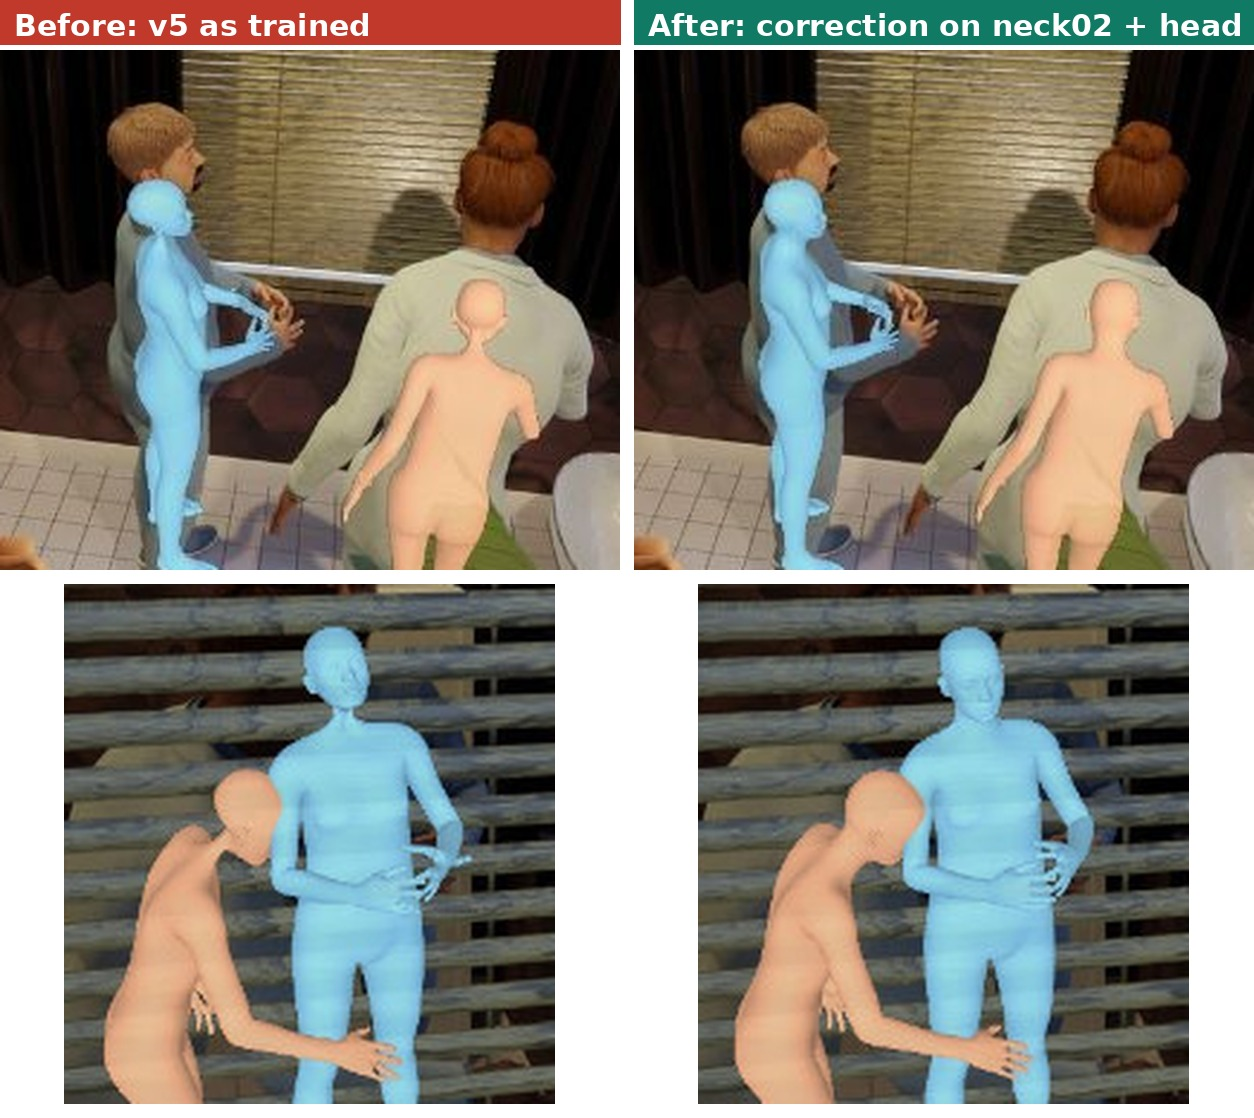
\includegraphics[width=0.62\linewidth]{figures/img/neck_before_after_v5.jpg}}%
  {\DiagPending{F6: holdout images 579862 and 579863, Base without and with the bone correction
   (docs/figures/neck\_before\_after\_v5.jpg)}}
\caption[The thin neck of Base, and the same checkpoint with the bone correction]{Holdout images 579862 (top) and
579863 (bottom). Left: Base as trained. Right: the same checkpoint with the output correction of
Section~\ref{sec:diag-neck}, no training; nothing else differs. Synthetic images, bodies at the model's own depth, so
the depth bug of Section~\ref{sec:diag-depth} still draws them too small. The correction also turns two hand bones;
only the necks were judged, by eye.}
\label{fig:neck-before-after-v5}
\end{figure}

Figure~\ref{fig:neck-before-after-v5} shows the first failure as it was seen. In the left column Base draws each neck
as a thin stalk, pinched under the head, on synthetic holdout images it never trained on. The second failure was the
hands: the predicted fingers curled into claws. From then on every real-photo demo set the fingers to rest pose. The
third failure was children. A standing boy in one of our own photos received an adult body
(Figure~\ref{fig:final-real-photos} shows him again with the final model).

The draft gave each failure a cause without a test against an alternative. For the neck it concluded that linear blend
skinning stretches the skin between Anny's stacked neck bones when the network predicts slightly different rotations
for each, ``a property of the rig, not a training failure''. A later reading blamed weak supervision on a redundant
four-bone chain, plus the depth defect. For the fingers the belief was resolution: a hand covers too few pixels. For
children the belief was that age had not been learned. The evidence was five small people in our own photos,
predicted at adult ages of \DiagSmallPeopleAgeLow{} to \DiagSmallPeopleAgeHigh. The rest of this chapter shows that the
neck explanation is wrong, that resolution explains little of the finger error, and that the child evidence was
wrong. Looked at again, four of the five ``small people'' were adults who crouched, sat or were cut off by the frame.
The skeletal height that had flagged them is measured on the posed body, so crouching shortens it, and their height
phenotype was \DiagSmallPeopleHeightLow{} to \DiagSmallPeopleHeightHigh, an adult rest body. Only the boy was a child.
He received age \DiagBoyAge{} and height phenotype \DiagBoyHeight: an adult body.

The figure does not show the fingers or the children, and it does not show a real photo; Chapter~\ref{ch:results}
has the real-image pairs. The neck widths are judged by eye; the number behind them is the neck girth of
Table~\ref{tab:neck}.

% -----------------------------------------------------------------------------
\section{What is not the cause: six structural checks}
\label{sec:diag-checks}

\begin{table}[tbp]
\centering\footnotesize
\begin{tabular}{@{}p{0.27\linewidth}p{0.2\linewidth}p{0.45\linewidth}@{}}
\toprule
check & sample & result \\
\midrule
1 ground truth decodes onto the people (no network) & manifest, 55 people &
labels render onto the people; \DiagGTInsideImage\,\% of joints inside the image, \DiagGTInsideBox\,\% inside the
box: the missing joints are truncation at the image border; dataset camera matches on 100\,\% of images \\
2 body model, rest pose and age sweep & body model only &
skeletal height \DiagAgeSweepLow\,m at age 0, \DiagAgeSweepHigh\,m at age 0.8; head/height
\DiagHeadRatioLow{} to \DiagHeadRatioHigh \\
3 single-joint moves & body model only &
all \DiagPerturbations{} pass (96--100\,\% of the moved vertices in the intended part); neck01 leaks about 4\,\% into
the shoulders, normal skinning \\
4 gradients and mesh response & 4 holdout images &
zero-gradient bones are exactly the \DiagHelperBones{} masked helpers; all \DiagActiveBones{} active bones and all
\DiagShapeOutputs{} shape outputs receive gradient; two of the three camera outputs receive none \\
5 prediction vs.\ truth; shape swap & holdout (\DiagHoldoutImages{} images, \DiagHoldoutPeople{} people), manifest &
neck length \DiagNeckLengthPct\,\% of truth; true shape with predicted pose lowers the PVE of the 10 manifest
children from \DiagChildSwapBefore{} to \DiagChildSwapAfter\,mm \\
6 capped overfit & 40 manifest training images, 400 steps &
training PVE \DiagOverfitTrainBefore{} $\to$ \DiagOverfitTrainAfter\,mm ($-$\DiagOverfitTrainDrop\,\%); holdout
\DiagOverfitHoldBefore{} $\to$ \DiagOverfitHoldAfter\,mm (+\DiagOverfitHoldRise\,\%); two warnings (text) \\
\bottomrule
\end{tabular}
\caption[Six structural checks]{Six structural checks on Base before any training change. The manifest is a fixed set
of 40 training images (10 adults, 10 children, 10 with visible hands, 10 hard neck poses) and 15 holdout images
(no children); it is excluded from every later fine-tune. Checks 1--5 are read-only; check 6 trains a throw-away copy
and reports setting V0 (helper bones unmasked).}
\label{tab:diag-checks}
\end{table}

\begin{figure}[tbp]
\centering
\IfFileExists{figures/img/gt_decode_overlay.jpg}%
  {\includegraphics[width=0.8\linewidth]{figures/img/gt_decode_overlay.jpg}}%
  {\DiagPending[0.8\linewidth]{F24: ground-truth decode overlay, AnnyOne labels rendered with the dataset camera
   (cluster: results/diagnostics/gt\_decode/vis/, two files)}}
\caption[Check 1: AnnyOne labels decoded and rendered with the dataset camera]{Check 1: AnnyOne ground-truth pose and
shape decoded through the same Anny body model as in training and drawn with the dataset camera, manifest images. No
network is involved; the meshes sit on the people.}
\label{fig:gt-decode}
\end{figure}

Table~\ref{tab:diag-checks} lists the six checks and Figure~\ref{fig:gt-decode} shows check~1. The ground truth decodes
onto the people. The share of joints inside the image and inside the annotated box move together per category, so
the missing joints are truncation, not a decoding error; the first automatic report called this a decoding defect
because its rule compared box containment with a fixed 95\,\%. The body model makes a child with child proportions,
and each of the 16 single-joint moves (neck and fingers among them) moves the intended part. The gradient check
found every active bone and every shape output reachable. Per bone the gradients range from \DiagGradRoot{} at the
root to \DiagGradFingers{} at the fingers, and the loss is dominated by shape (\DiagLossShareShape\,\%), while the
translation and distance terms take \DiagLossShareTransl\,\% and \DiagLossShareDist\,\%. On the holdout the predicted
neck has the right length, and predicted shape explains the small remainder. The capped overfit lowered the training
error by a third and raised the holdout error, as memorising must.

Read together, the checks rule out the rig, the decoding of the labels and the gradient path. The draft's four neck
tests stay valid as eliminations of the same kind: the rest-pose render looked normal, all neck bones are active in
the loss, the thin neck appears on synthetic images, and the proportions phenotype is accurate. So the cause had to be
in what training asked the network to do. The overfit test gave two warnings. First, the summed rotation loss barely
moved while the images were memorised (\DiagOverfitRotFirst{} $\to$ \DiagOverfitRotLast). Second, the translation and
2D reprojection terms rose (\DiagOverfitTranslFirst{} $\to$ \DiagOverfitTranslLast{} and \DiagOverfitTwoDFirst{}
$\to$ \DiagOverfitTwoDLast, first against last five epochs) while the pelvis-centred 3D terms fell. This was possibly a
first sign of the depth bug of the next section. It is weak evidence: each value is a single-batch print, and the
averages of the first and second half fall instead (\DiagOverfitTranslHalfA{} $\to$ \DiagOverfitTranslHalfB{} and
\DiagOverfitTwoDHalfA{} $\to$ \DiagOverfitTwoDHalfB).

The checks cannot see two kinds of fault. A target that is consistent in itself but placed at a different joint
than the model's anchor passes every check, because the checks compare pelvis-centred quantities. A bone that is
flipped the same way in every person passes too, because the checks tested the rig in isolation and averaged the
bone errors by group. Both faults were there. The holdout also has no children, so every child number in this chapter
is in-sample or from real photos.

% -----------------------------------------------------------------------------
\section{The hidden depth bug}
\label{sec:diag-depth}

\begin{table}[tbp]
\centering\footnotesize
\begin{tabular}{@{}lrr@{}}
\toprule
quantity & truth & Base \\
\midrule
pelvis depth, mean (sd)                                & \DiagDepthTrueMean\,m (\DiagDepthTrueSd) & \DiagDepthPredMean\,m (\DiagDepthPredSd) \\
linear fit of predicted on true depth                  & slope 1, intercept 0 & slope \DiagDepthSlopeBase, intercept \DiagDepthInterceptBase\,m \\
people predicted farther than truth                    & --                  & \DiagDepthFartherPct\,\% \\
correlation of true depth with depth error             & --                  & \DiagDepthCorrError \\
skeletal height (3D, metric)                           & \DiagSkelHeightTrue\,m & \DiagSkelHeightPred\,m ($r = \DiagSkelHeightCorr$) \\
drawn size, predicted over true (pixels)               & 1                   & \DiagSizeBase \\
pelvis root error (3D)                                 & 0                   & \DiagRootErrBase\,m \\
head / pelvis 2D error, median (mean)                  & 0                   & \DiagHeadPxBaseMedian{} (\DiagHeadPxBase) / \DiagPelvisPxBaseMedian{} (\DiagPelvisPxBase) px \\
correlation of PVE with depth error                    & --                  & \DiagCorrPVEDepth \\
\bottomrule
\end{tabular}
\caption[Placement of Base on the holdout]{Where Base places people. V1, 100-image AnnyOne holdout, all
\DiagHoldoutPeople{} matched people. The body has the right metric size but is placed too far away, so it is drawn
too small; PVE, which aligns the pelvis first, does not see it.}
\label{tab:diag-placement}
\end{table}

% T08 Depth fix: the depth-anchor pilots, the final model and its control (REWRITE_PLAN.md section 4, T8).
% Owner: Diagnostics writer (chapter 5, section "The hidden depth bug"); also referenced from Results 6.2.
% Setting: V1, 100-image AnnyOne holdout (579,860-579,959), matched people; root error = PLACEMENT table `root mm`
% (absolute 3D pelvis distance), never the signed `root dz`.
% Sources (handover.md 3.1 tables, checked against the logs there; head px from the deck build
% docs/deck_src/build.js:439, slide 14, and handover 3.1 for the final model and control):
%   Base (v5 00099)           3571596:55,64; 3570222:40
%   2-ep control              3571599:49,58,67-68   (pilot_root_dist1_transl1_...)
%   2-ep fix x1               3571598:66,75,84-85   (pilot_person_center_dist1_transl1_...)
%   2-ep fix x5               3572418:52,61,70-71
%   2-ep fix x20              3572483:57,66,75-76
%   10-ep control             3571934:134,143,152-153 (long_root)
%   10-ep fix x1              3571933:125,134,143-144 (long_person_center)
%   10-ep fix x5              3572482:126,135,144-145 (long_pc_dist5)
%   Control (exp7)            3611339:166,175,182-184; head px 67.1 (3611339:166)
%   Final (exp7 fix arm)      3611336:175,184,191-193; head px 7.6 (3611336:175)
%   Mixed-L e62 3571963:40,55,64; Fresh-heads-L (v10 e290) 3571794:40,55,64 (no head px quoted)
% PVE / recall rounded to one decimal from the handover's two-decimal values (72.19 -> 72.2, 77.25 -> 77.3 as on the deck).
\begin{table}[htbp]
\centering\footnotesize
\setlength{\tabcolsep}{3pt}
\begin{tabular}{@{}lrrrrrrrr@{}}
\toprule
run (depth loss) & root (m) & size & slope & icpt.\ (m) & head px & pelvis px & PVE & recall \\
\midrule
Base & 1.21 & 0.63 & 0.33 & 2.36 & 64.5 & 23.4 & 70.5 & 90.2 \\
\addlinespace
\multicolumn{9}{@{}l}{\emph{2-epoch fine-tunes of Base, AnnyOne only}} \\
control $\times$1 & 1.11 & 0.66 & 0.33 & 2.28 & 58.1 & 23.3 & 72.3 & 89.8 \\
fix $\times$1 & 0.69 & 0.78 & 0.30 & 1.93 &  9.6 & 37.3 & 77.3 & 87.8 \\
fix $\times$5 & 0.66 & 0.80 & 0.44 & 1.62 &  8.5 & 38.1 & 76.8 & 87.8 \\
fix $\times$20 & 0.53 & 0.87 & 0.43 & 1.44 &  8.8 & 31.4 & 75.7 & 87.4 \\
\addlinespace
\multicolumn{9}{@{}l}{\emph{10-epoch fine-tunes of Base, AnnyOne only}} \\
control $\times$1 & 1.44 & 0.59 & 0.34 & 2.59 & 64.0 & 24.3 & 72.2 & 89.4 \\
fix $\times$1 & 0.73 & 0.78 & 0.30 & 1.98 &  7.6 & 38.5 & 75.5 & 87.0 \\
fix $\times$5 & 0.54 & 0.84 & 0.38 & 1.59 &  7.2 & 33.1 & 74.8 & 87.8 \\
\addlinespace
\multicolumn{9}{@{}l}{\emph{10-epoch fine-tunes of Base with 30\% 3DPW (v23 labels)}} \\
Control $\times$1 & 1.40 & 0.59 & 0.28 & 2.66 & 67.1 & 26.7 & 77.4 & 89.0 \\
Final $\times$5 & 0.73 & 0.78 & 0.42 & 1.75 &  7.6 & 41.1 & 73.7 & 87.0 \\
\addlinespace
\multicolumn{9}{@{}l}{\emph{other checkpoints trained with pelvis targets}} \\
Mixed-L & 1.39 & 0.59 & 0.31 & 2.60 &  --  & 25.1 & 75.0 & 88.6 \\
Fresh-heads-L & 1.49 & 0.57 & 0.28 & 2.71 &  --  & 24.0 & 74.1 & 89.0 \\
\bottomrule
\end{tabular}
\caption[Depth fix: pilots, final model and control]{Placement before and after building the training targets at
the head joint. V1, 100-image AnnyOne holdout, matched people. Root error: absolute 3D distance of the pelvis; size:
predicted over true head-to-pelvis distance in pixels (1 is right); slope and intercept: linear fit of predicted
against true pelvis depth (1 and 0\,m are right); head and pelvis px: 2D error of those joints; PVE in mm, recall in \%. Control
rows build the targets at the pelvis, fix rows at the head; $\times$1/5/20: weight of the distance and translation
terms. Final also has the bone correction. One run per row, no seed. No control was run at
$\times$5 or $\times$20; each fix row is read against the control of the same length.}
\label{tab:depth-runs}
\end{table}


Table~\ref{tab:diag-placement} is the placement section of the holdout trace. True pelvis depths average
\DiagDepthTrueMean\,m; Base predicts \DiagDepthPredMean\,m with a smaller spread. A straight-line fit gives predicted
$= \DiagDepthSlopeBase \times \text{true} + \DiagDepthInterceptBase$\,m (Figure~\ref{fig:depth-scatter}). All
\DiagHoldoutPeople{} people are placed too far, and the nearest are pushed farthest (correlation
\DiagDepthCorrError). The 3D skeleton has the right height, so a body of the right size sits at the wrong distance and
is drawn at \DiagSizeBase{} of its true size. Its pelvis lands near the right pixel, its head does not. PVE is blind to
all of this: its correlation with the depth error is \DiagCorrPVEDepth.

The trace was not the only sign. The gradient check had shown that two of the three camera outputs receive no
gradient, and the overfit test had shown the translation and 2D terms rising. A read of the training code gave the
mismatch. The model places each mesh by its head joint and reports the head as its
position, but the training code built the translation, distance, detection-cell and offset targets at joint 0, the
pelvis. A one-batch debug print confirmed it: the predicted vertical offsets were \DiagOffsetMin{} to
\DiagOffsetMax{} cells where the legal range is $\pm$0.5. The likely mechanism, which I did not test on its own, is
this. The detection and offset terms pull the anchor pixel toward the pelvis, while the mesh hangs from that pixel by
its head, so every projected joint is displaced by the head-to-pelvis distance in pixels. The 2D terms are the only
strong terms that see depth, because the 3D joint and vertex terms are pelvis-centred. They can shrink the
displacement only by drawing the body smaller, that is, by predicting it farther away. The distance and translation
terms, \DiagLossShareDepthTerms\,\% of the loss, could not resist. Near people have the largest head-to-pelvis
distance in pixels and were pushed farthest, which matches the correlation above. Building the targets at the head
(Chapter~\ref{ch:method}) is the fix; Table~\ref{tab:depth-runs} is its test.

In Table~\ref{tab:depth-runs} all five fix runs reach a root error of \DiagRootErrFixLow--\DiagRootErrFixHigh\,m, and
both pelvis-target controls with the same schedule stay at \DiagRootErrCtrlLow--\DiagRootErrCtrlHigh\,m. The drawn size
rises from \DiagSizeCtrlLow--\DiagSizeCtrlHigh{} to \DiagSizeFixLow--\DiagSizeFixHigh, and the head lands within 7 to
10 pixels instead of 58 to 67. The final model keeps the fix with 30\,\% real images and the bone correction in
training: root error \DiagFinalRootErr{} against \DiagControlRootErr\,m for its Control, size \DiagFinalSize{} against
\DiagControlSize, slope \DiagFinalSlope{} against \DiagControlSlope. These gaps are far above the run-to-run variation:
every fix run lies below every control. Two checkpoints trained with pelvis targets, Base+3DPW (old labels) and a
fresh-head run, carry the same bug (\DiagOldRootErrA{} and \DiagOldRootErrB\,m). The bug stayed hidden for two reasons.
PVE and PA-PVE align the pelvis before measuring. The real-photo demos place every body from its detection box, so
only the synthetic demo and the trace panels ever used the model's own depth.

The table does not show a solved depth. The fix moved the offset and the body size, not the slope (Final: \DiagFinalSlope): \DiagSlopeSwitch{}
with the switch alone and \DiagSlopeStrongLow--\DiagSlopeStrongHigh{} with a stronger depth loss, far from 1.
Predictions are still pulled toward about 2.5 to 2.9\,m, for a reason I have not found. The pelvis 2D error rose from
about 23 to 31--41 pixels; the likely reason is that the head is now pinned while the body is still drawn too small,
which was not checked. Every fix run is also worse than its control on PVE (+\DiagFixCostPVELow{} to
+\DiagFixCostPVEHigh\,mm) and recall ($-$\DiagFixCostRecallLow{} to $-$\DiagFixCostRecallHigh{} points). Each gap is
within run-to-run variation, but all five point the same way, so I report them as a likely cost. By the success rule
written before the pilots ran (PVE at most 71.5\,mm and recall at least 89.2\,\%), every run failed, the controls
included.

% -----------------------------------------------------------------------------
\section{The neck: a per-bone dump}
\label{sec:diag-neck}

\begin{table}[tbp]
\centering\footnotesize
\begin{tabular}{@{}lrrrl@{}}
\toprule
bone & local error (deg) & global error (deg) & verdict & note \\
\midrule
neck01 & \DiagDumpNeckOne   & --    & OK          & \\
neck02 & \DiagDumpNeckTwo   & --    & half-turn   & twist \DiagDumpNeckTwoTwist\,deg about its own axis, swing \DiagDumpNeckTwoSwing\,deg \\
neck03 & \DiagDumpNeckThree & \DiagDumpNeckThreeGlobal & OK locally & carries neck02's turn \\
head   & \DiagDumpHead      & \DiagDumpHeadGlobal      & half-turn   & turns the chain back \\
jaw    & \DiagDumpJaw       & --    & OK          & \\
\bottomrule
\end{tabular}
\caption[Per-bone dump of the neck chain]{Per-bone dump of Base's neck chain. V1, 100-image AnnyOne holdout,
\DiagHoldoutPeople{} people; medians. Local error: relative to the parent bone; global error: of the bone's orientation
in the camera frame. A half-turn is an error above 150\,deg in at least half the people.}
\label{tab:diag-neck-dump}
\end{table}

% T09 Neck: the bone correction without training, with a 2-epoch fine-tune, and in the final model
% (REWRITE_PLAN.md section 4, T9). Owner: Diagnostics writer (5.4); also referenced from Results 6.3.
% Setting: V1, 100-image AnnyOne holdout, 222 people, matched people.
% Sources: columns 1-4 = exp6 on v5, job 3579014:101-114 (handover 3.2 table and 0b);
%          column 5 = exp7 control 3611339:182-198; column 6 = final model 3611336:191-207 (handover 3.2, 5/7).
% Rows: neck02 :101 / :193,:197 / :202,:206; head :103 / :194,:198 / :203,:207; metacarpal1.L, finger4-1.R :105-106 /
%   3611339:195-196 / 3611336:204-205; girth :107 / :189 / :198; PVE_neck :108 / :190 / :199; PVE :109 / :182 / :191;
%   PA-PVE :110; recall :112; global head :113 / :191 / :200; fingers :114 / :192 / :201.
% "not dumped" = the holdout dump 3573518 did not cover finger bones; finger4-1.R was found on the training images.
% Correction constants 178.8 / 179.2 / 179.8 / 179.7 deg (3579014:12, :37), from 200 training images.
\begin{table}[htbp]
\centering\footnotesize
\setlength{\tabcolsep}{3pt}
\newcommand{\hd}[1]{\begin{tabular}[b]{@{}c@{}}#1\end{tabular}}
\begin{tabular}{@{}lrrrrrr@{}}
\toprule
 & \hd{Base} & \hd{corr.,\\no train.} & \hd{corr.\ +\\2-ep.\ FT} & \hd{2-ep.\\control}
 & \hd{Control\\10 ep.} & \hd{Final\\10 ep.} \\
\midrule
neck02 (deg)         & 175.6 &   4.5 &   4.7 & 175.7 & 175.8 &   4.8 \\
head bone (deg)      & 177.9 &  12.4 &  11.2 & 177.9 & 177.7 &   8.9 \\
metacarpal1.L (deg)                 & 180.0 &   0.0 &   0.0 &  --   & 180.0 &   0.0 \\
finger4-1.R (deg)                   & n.d.  &  10.2 &  10.3 &  --   & 180.0 &   9.6 \\
neck girth, pred./true& 0.461 & 1.004 & 0.997 & 0.461 & 0.464 & 0.996 \\
PVE$_\text{neck}$ (mm) & 27.3 & 10.8 & 10.7 & 27.9 & 27.7 & 11.0 \\
\addlinespace
body PVE (mm)                       &  70.5 &  71.3 &  68.8 &  76.9 &  77.4 &  73.7 \\
PA-PVE (mm)                         &  53.3 &  52.2 &  50.9 &  55.2 &  56.4 &  50.3 \\
recall (\%)                         &  90.2 &  90.2 &  89.4 &  91.1 &  89.0 &  87.0 \\
head direction (deg)         &  12.0 &  19.1 &  14.4 &  13.8 &  13.0 &  13.1 \\
fingers (deg)                       &  17.3 &   8.2 &   8.3 &  17.4 &  17.4 &   8.3 \\
\bottomrule
\end{tabular}
\caption[Neck: the half-turned bones and their correction]{The two half-turned neck bones and their correction. V1,
100-image AnnyOne holdout, matched people. Bone errors are local (relative to the parent bone) medians; about 180\,deg
means the bone is turned half a turn. Girth: radius of the neck skin, predicted over true. PVE$_\text{neck}$: vertex
error over the 171 neck-skin vertices, centred at neck01. Corr.: one constant rotation per flipped bone
(neck02, head, metacarpal1.L, finger4-1.R), estimated on 200 training images. FT: fine-tune. The 2-epoch columns are AnnyOne-only fine-tunes of Base; Control and Final are the 10-epoch runs with 30\% 3DPW, Final also with the depth fix. n.d.: not
dumped on the holdout. One run per column, no seed; PVE gaps below about 10\,mm are within run-to-run variation
(Table~\ref{tab:pilot-noise}).}
\label{tab:neck-bones}
\end{table}


Table~\ref{tab:diag-neck-dump} is the dump that found the neck fault. neck02 is wrong by \DiagDumpNeckTwo\,deg, a
half-turn about its own axis, and the head bone by \DiagDumpHead\,deg. neck03 is right relative to its parent but
\DiagDumpNeckThreeGlobal\,deg off in the camera frame, because it inherits neck02's turn. The two half-turns cancel, so
the head points the right way (\DiagDumpHeadGlobal\,deg) and PVE never showed the fault. The skin between them is
twisted thin: the neck girth is \DiagNeckGirthBase{} of the truth and the neck-skin error \DiagNeckSkinBase\,mm
(Table~\ref{tab:neck}). The earlier figures of 62.7\,deg for the neck and 89.5\,deg for the head were group means
over these bones; they hid the flip and suggested weak supervision. The same flip is in all eight checkpoints of the
Base line: the three training stages before Base, Base, Base+3DPW, the 10-epoch depth-fix pilot and two pilots with
a geodesic rotation loss (neck02 \DiagNeckTwoRangeLow--\DiagNeckTwoRangeHigh\,deg, girth
\DiagGirthRangeLow--\DiagGirthRangeHigh). It is present from the first stage, which trained fresh heads on a frozen
backbone, before the helper mask, the neck boost and the shape weight of 20 were introduced. The depth-fix pilot keeps
girth \DiagGirthRangeLow, so depth is not the cause of the neck. A fresh-head run started from the same pretrained
backbone has a normal neck (girth \DiagFreshGirth, neck-skin error \DiagFreshNeckSkin\,mm), but flips other bones: a
compensated pair in the left arm (shoulder01.L and upperarm02.L) and three metacarpals.

This refutes the draft's explanation. The rig is fine: all 16 single-joint moves pass. The rest-pose render, which had
seemed to support skin stretch, is explained just as well by the flip, because rest pose sets every rotation to the
identity and so removes both half-turns. Only the per-bone dump separates the two explanations. The ground-truth
rotation blocks are all proper rotations, and every checkpoint uses the same local-bone pose parameterisation. A loss
weight cannot undo a half-turn. The neck boost of the earlier stage is $\times$2.41 for the boosted bones and
$\times$0.60 for the rest after renormalisation, and it left the neck unchanged. A geodesic rotation loss moved neck02
only from \DiagNeckTwoBase{} to \DiagGeodesicNeckTwo\,deg in 2 epochs. The likely reason is that neck02 and the head
must turn back together, and any partial turn raises the loss. So I corrected the output instead: one constant
rotation $C_b$ per flipped bone, applied as $R_b \leftarrow R_b C_b$ after the rotation decoding, estimated on 200
training images and never on the holdout (Chapter~\ref{ch:method}). The constants are \DiagCorrNeckTwo,
\DiagCorrHead, \DiagCorrMetacarpal{} and \DiagCorrFinger\,deg for neck02, head, metacarpal1.L and finger4-1.R.

Table~\ref{tab:neck} reads as follows. Without training the correction turns neck02 back to \DiagNeckTwoNoTrain\,deg
and restores the girth (\DiagGirthNoTrain) and the neck-skin error (\DiagNeckSkinNoTrain\,mm). The head direction gets
worse, \DiagHeadDirBase{} to \DiagHeadDirNoTrain\,deg, above the 15-degree limit set before the run. The likely reason
is the compensated chain: the head's error differs from person to person, so one constant cannot undo it. After a
2-epoch fine-tune with the correction in place the head direction is \DiagHeadDirFineTune\,deg, against
\DiagHeadDirCtrlTwo\,deg for the control, which keeps the flip. Body PVE reads \DiagPVEBase{}, \DiagPVENoTrain{} and
\DiagPVEFineTune\,mm against \DiagPVECtrlTwo\,mm for the control. That gap is within run-to-run variation, and the
control sits above the range of six earlier arms, so the result is no sign of a PVE cost, not a gain. The final model
keeps the correction through 10 epochs with real images: neck02 \DiagFinalNeckTwo\,deg, head \DiagFinalHeadBone\,deg,
girth \DiagFinalGirth, neck-skin error \DiagFinalNeckSkin\,mm, head direction \DiagFinalHeadDir{} against
\DiagControlHeadDir\,deg for Control.

\begin{figure}[tbp]
\centering
\begin{subfigure}[t]{0.48\linewidth}\centering
\IfFileExists{figures/img/exp6_compare_579864.jpg}%
  {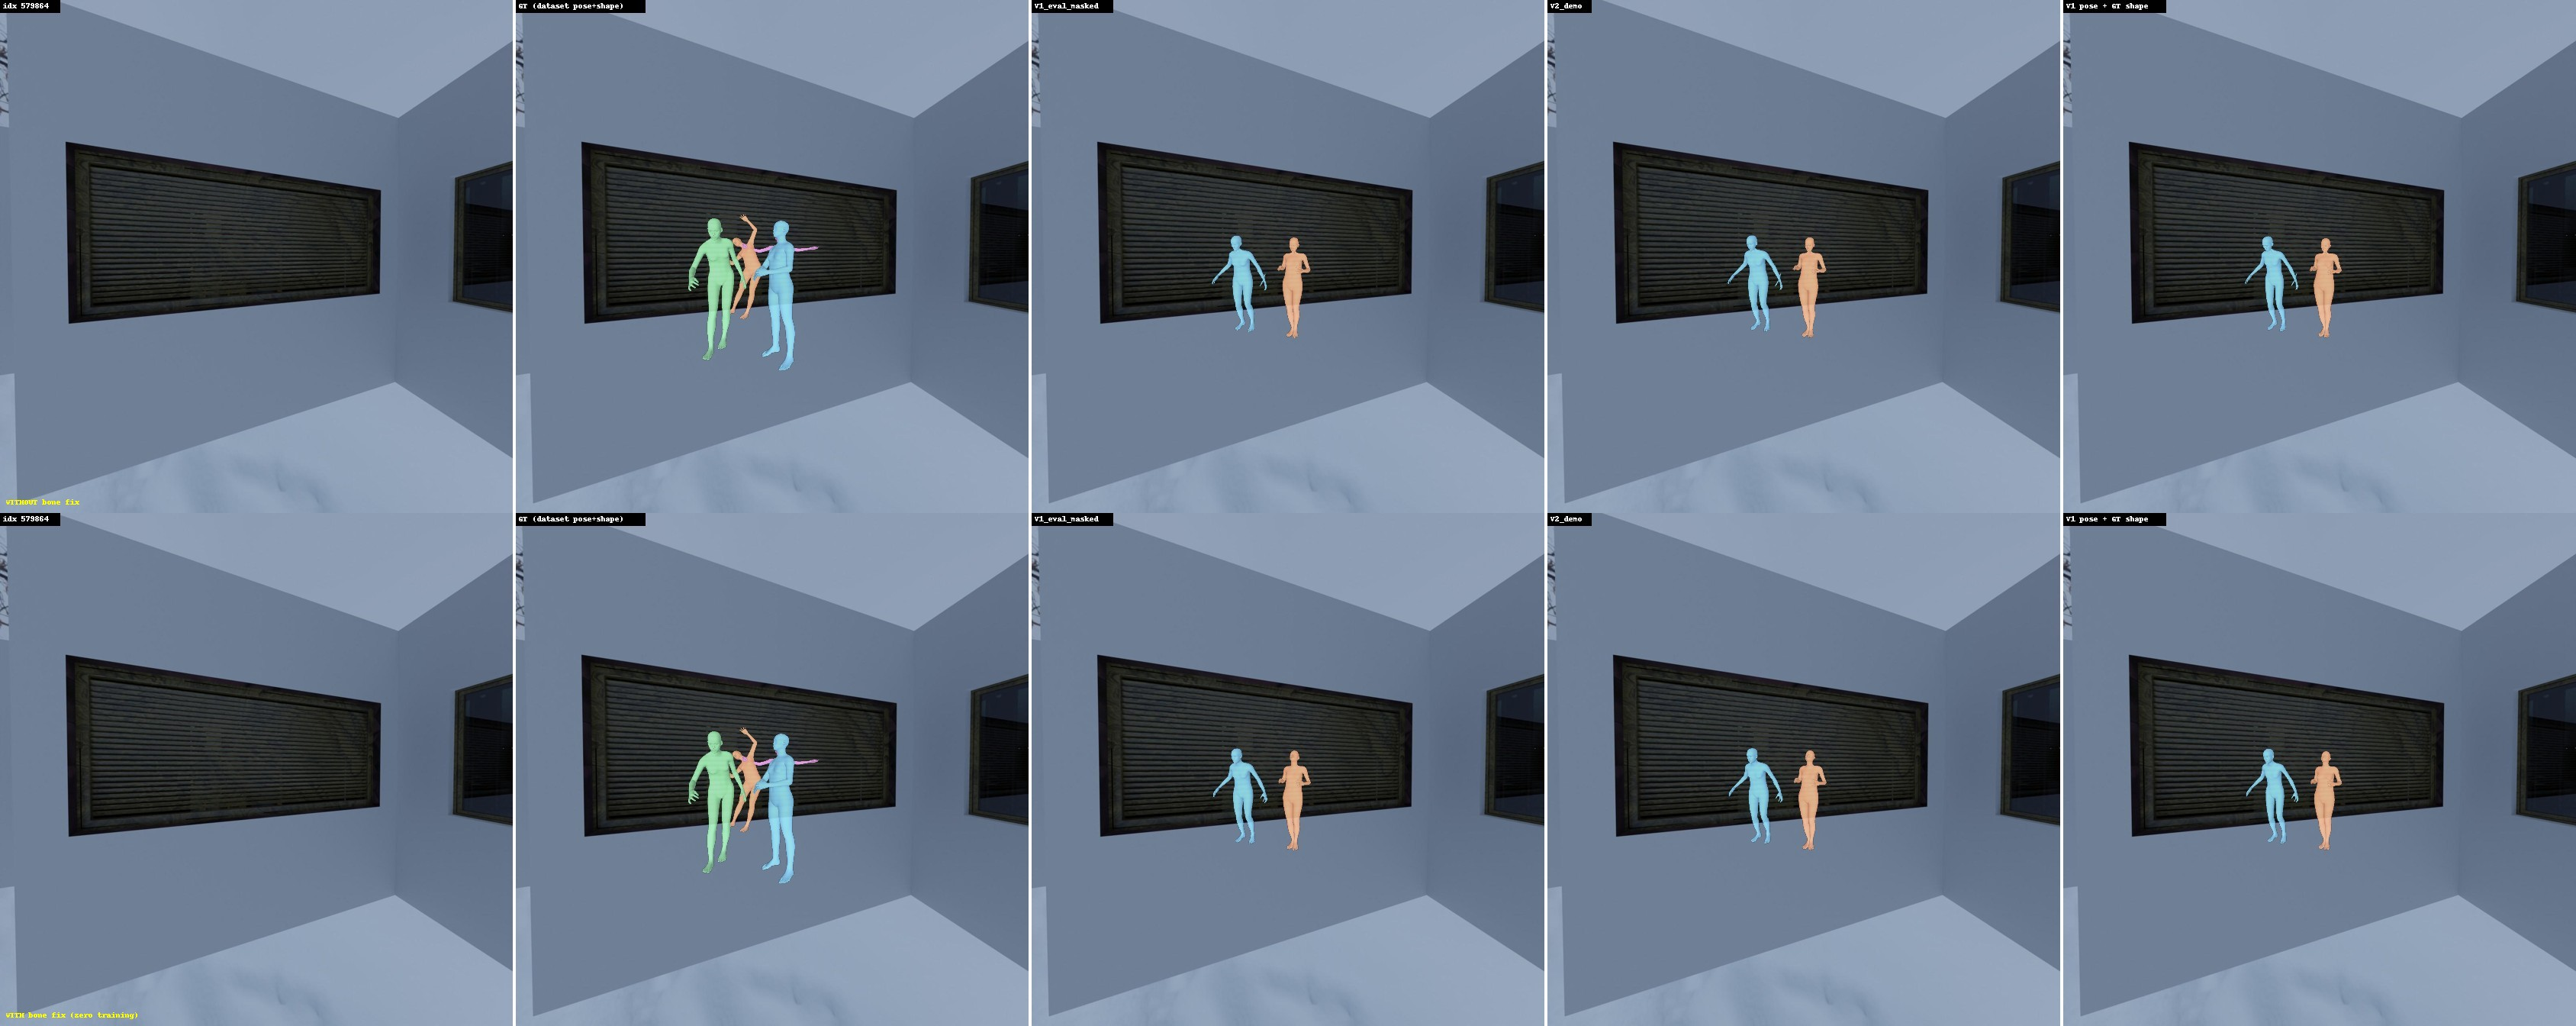
\includegraphics[width=\linewidth]{figures/img/exp6_compare_579864.jpg}}%
  {\DiagPending[0.95\linewidth]{F23a: holdout 579864, without (top) and with (bottom) the correction
   (cluster: exp6 compare/579864.jpg)}}
\caption{holdout image 579864}
\end{subfigure}\hfill
\begin{subfigure}[t]{0.48\linewidth}\centering
\IfFileExists{figures/img/exp6_compare_579866.jpg}%
  {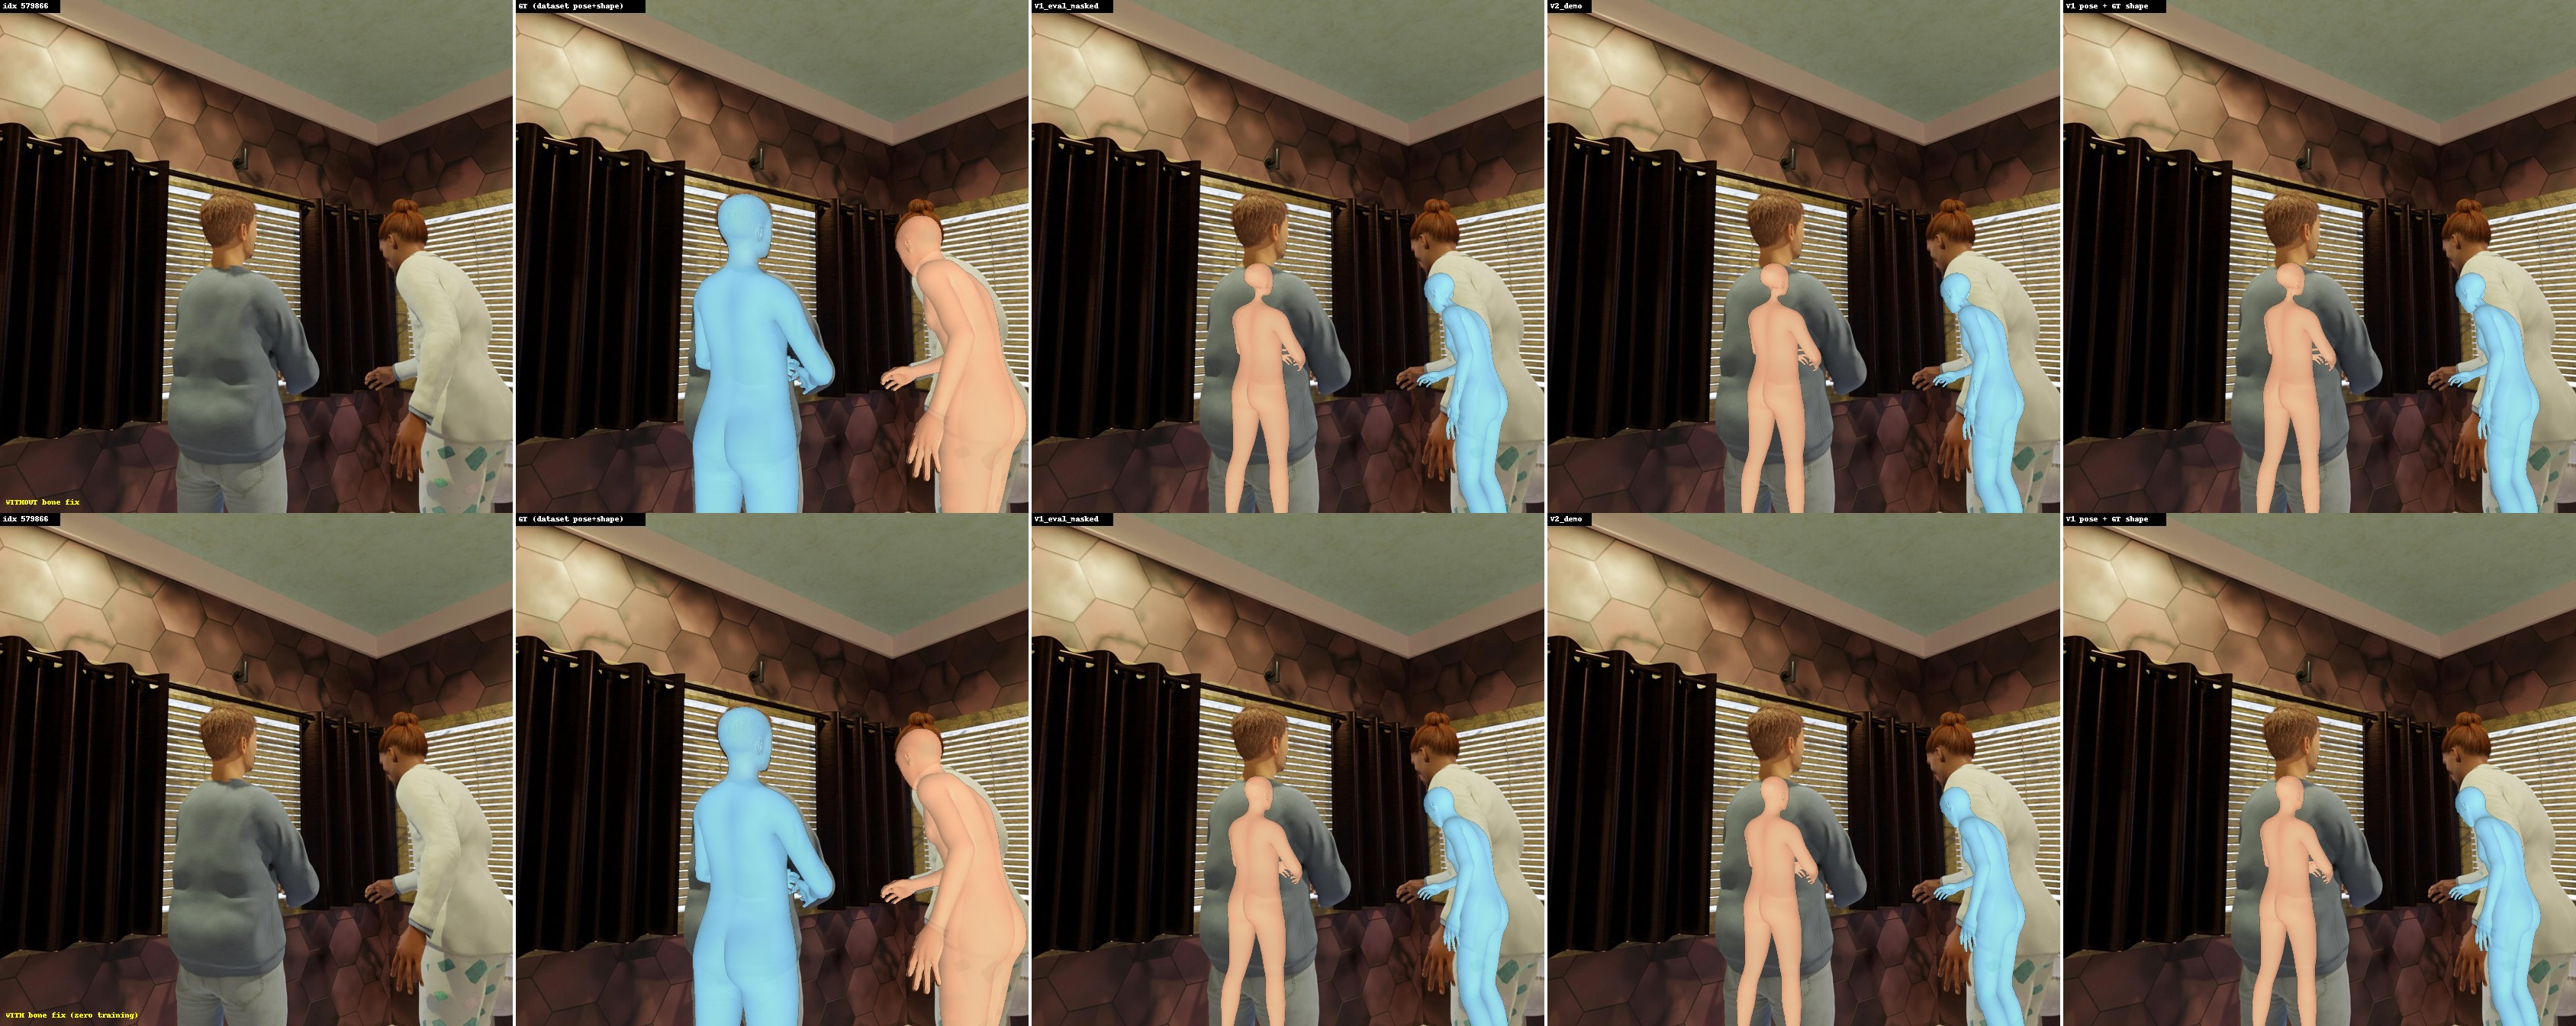
\includegraphics[width=\linewidth]{figures/img/exp6_compare_579866.jpg}}%
  {\DiagPending[0.95\linewidth]{F23b: holdout 579866, without (top) and with (bottom) the correction
   (cluster: exp6 compare/579866.jpg)}}
\caption{holdout image 579866}
\end{subfigure}
\caption[Bone correction on two more holdout images]{Two more holdout images, Base without (top row) and with
(bottom row) the bone correction, no training, bodies at the model's own depth. Synthetic; judged by eye; the depth
bug is still present.}
\label{fig:exp6-compare}
\end{figure}

What is not shown: why the bones flipped. The 6D start value of the rotation output is singular and starts a bone
tilted about its local $x$ axis; that fits the tilted metacarpal1.L but not the twist of neck02, so the origin is
unknown. The correction adds no parameters, and it says nothing about the origin. A two-sided correction, needed to
keep a compensated chain such as the fresh-head run's left arm intact, was not implemented. On real photos there is no
neck ground truth; the real-image pairs (Figure~\ref{fig:neck-3dpw}) are judged by eye, and there the fixed model also
had the 2-epoch fine-tune.

% -----------------------------------------------------------------------------
\section{The fingers}
\label{sec:diag-fingers}

% T10 Fingers (REWRITE_PLAN.md section 4, T10). Owner: Diagnostics writer (5.5); also referenced from Results 6.4.
% Setting: V1, 100-image AnnyOne holdout, matched people; finger error = mean local rotation error over the finger bones.
% Sources: predicted 17.3 / rest 15.1 (3571960:290; findings "Fingers"); test-time crop x1.3 17.2, body PVE 124.8
%   (3571960:294-299); region-normalised loss 17.5 vs control 17.4 (3571959:316; 3571960:314); bone correction no
%   training 8.2 (3579014:114); + 2-ep fine-tune 8.3 (3579014:114); final 8.3 vs control 17.4 (3611336:201;
%   3611339:192); Fresh-heads-L (v10) three metacarpals 32.0 -> 17.8 (3579015:80).
%   Hand size: 2.25 tokens median at 672 px, 41% under 2 tokens (3571960:287); person crop 4.2 / 0%, children's hands
%   0.7 / 80% (deck slide 17, D slide 17).
%   Hands' share of the rotation loss ~70% (with x4 boost) -> 33% (deck notes slide 17, handover 3.3).
\begin{table}[!htb]
\centering\footnotesize
\begin{tabular}{@{}lrr@{}}
\toprule
\multicolumn{3}{@{}l}{\emph{(a) finger rotation error on the holdout}} \\
setting & fingers (deg) & reference (deg) \\
\midrule
Base, predicted fingers                                   & 17.3 & -- \\
Base, fingers set to rest pose                             & 15.1 & -- \\
Base, test-time person crop (PVE 124.8\,mm) & 17.2 & 17.3 (paired) \\
region-normalised rotation loss, 2 ep. & 17.5 & 17.4 (control) \\
Base + bone correction, no training                        &  8.2 & 17.3 (Base) \\
Base + bone correction, 2-ep.\ fine-tune &  8.3 & 17.4 (control) \\
Final (10 ep., 30\% 3DPW)                                  &  8.3 & 17.4 (Control) \\
Fresh-heads-L, three metacarpals corrected & 17.8 & 32.0 (uncorr.) \\
\midrule
\multicolumn{3}{@{}l}{\emph{(b) hand size in tokens (14-px patches of the 672-px input)}} \\
 & median length & under 2 tokens \\
\midrule
full image, all hands       & 2.25 & 41\% \\
person crop at test time    & 4.2  &  0\% \\
children's hands, full image & 0.7  & 80\% \\
\bottomrule
\end{tabular}
\caption[Fingers: what changed the finger error]{Fingers. (a) Finger rotation error, V1, 100-image AnnyOne holdout,
matched people; the reference is the matching run without the change. Rest pose keeps the metacarpals predicted, so
the 15.1\,deg still contains the flipped metacarpal1.L. (b) Hand length in input tokens. One run per row, no seed.}
\label{tab:fingers}
\end{table}


Table~\ref{tab:fingers} collects every finger measurement. Predicted fingers are \DiagFingersBase\,deg off; fingers set
to rest pose are \DiagFingersRest\,deg off, so the prediction was worse than no prediction. Hands are small: the
median hand is \DiagHandTokens{} tokens long in the 672-pixel input and \DiagHandUnderTwo\,\% of hands are shorter than
two tokens. A person crop at test time raises the median to 4.2 tokens, but the finger error stays at \DiagFingersZoom\,deg
while body PVE nearly doubles to \DiagZoomPVE\,mm, because the model never saw such a camera. A region-normalised
rotation loss gave \DiagFingersRegion\,deg against \DiagFingersRegionCtrl\,deg for its control. The per-bone search on
200 training images then found two hand bones turned half a turn, metacarpal1.L (180\,deg) and finger4-1.R
(178.8\,deg). Correcting them lowers the finger error to \DiagFingersFixNoTrain\,deg without training and
\DiagFingersFixFT\,deg after the fine-tune; the final model holds \DiagFingersFinal{} against
\DiagFingersControl\,deg for Control.

About half the finger error was therefore two flipped bones, not resolution. The resolution belief was tested only by
test-time zoom, which did not help; a hand-crop branch was never tested. The region-normalised loss cut the hands'
share of the rotation loss from about 70\,\% (with the neck and hand boost) to 33\,\%, so it was a rebalance, not an
upweighting. The gradient check had shown the smallest gradients of any bone group at the fingers and the worst
conditioning of their 6D outputs; whether the fingers are also under-trained is a guess I did not test.

Predicted fingers have not been shown on a real photo: every demo so far sets them to rest pose. Rest pose keeps the
metacarpals predicted, so the \DiagFingersRest\,deg still contains the metacarpal1.L flip, and a rest-pose floor with
the correction was not measured. The split of the 9.1-degree drop between the two bones was not measured either.

% -----------------------------------------------------------------------------
\section{Children and body shape}
\label{sec:diag-children}

% T18 Shape head: shape weight 1 vs 20, plus the regression to the median in the tails
% (REWRITE_PLAN.md section 4, T18). Owner: Diagnostics writer (5.6).
% Part (a): the draft's tab:shape as is (main.tex:980-998), n = 10 holdout images (plan 1.7); "fixed" softened to
%   "near the mode"; v4 = the stage before Base (alpha_shape 1, boosted_v4 00299), v5 = Base (alpha_shape 20).
% Part (b): holdout GT age 0.6-0.8 (n = 53, mean 0.67) predicted 0.57 (3570222:89); full holdout near the mode
%   age bias -0.015 / abs 0.037, gender -0.008 / 0.068 (3570222:75); in-sample babies (youngest 50, GT age 0.015)
%   predicted 0.10 (3569950:61; 3571955:174-175), height -0.25 traded (3569950:61,76); training medians gender 0.588,
%   age 0.601, height 0.500 (3569948:8-18); holdout youngest person 0.513 (3569948:33).
\begin{table}[htbp]
\centering\footnotesize
\begin{tabular}{@{}lrrrrl@{}}
\toprule
\multicolumn{6}{@{}l}{\emph{(a) predicted minus true phenotype, 10 holdout images (draft measurement)}} \\
phenotype & true mean & true std & weight 1 & weight 20 (Base) & reading \\
\midrule
age         & 0.553 & 0.036 & $+0.199$ & $-0.002$ & near the mode \\
height      & 0.579 & 0.026 & $-0.154$ & $-0.026$ & near the mode \\
proportions & 0.763 & 0.070 & $-0.017$ & $-0.001$ & near the mode \\
firmness    & 0.757 & 0.039 & $-0.167$ & $-0.190$ & unchanged \\
gender      & 0.694 & --    & $-0.042$ & $-0.063$ & $\approx$ \\
weight      & 0.382 & --    & $+0.056$ & $+0.064$ & $\approx$ \\
\midrule
\multicolumn{6}{@{}l}{\emph{(b) Base on the full holdout and in the young tail}} \\
\multicolumn{3}{@{}p{0.47\linewidth}}{holdout, all 222 people (nobody younger than 0.513)} & \multicolumn{3}{p{0.38\linewidth}}{age bias $-0.015$ (abs.\ 0.037); gender $-0.008$ (0.068)} \\
\multicolumn{3}{@{}p{0.47\linewidth}}{holdout, true age 0.6--0.8 ($n = 53$, mean 0.67)} & \multicolumn{3}{p{0.38\linewidth}}{predicted age 0.57} \\
\multicolumn{3}{@{}p{0.47\linewidth}}{50 youngest training people (in-sample, true age 0.015)} & \multicolumn{3}{p{0.38\linewidth}}{predicted age 0.10; height $-0.25$} \\
\multicolumn{3}{@{}p{0.47\linewidth}}{training medians (AnnyOne)} & \multicolumn{3}{p{0.38\linewidth}}{gender 0.588, age 0.601, height 0.500} \\
\bottomrule
\end{tabular}
\caption[Shape head: shape weight and the pull to the median]{Shape head. (a) The draft's comparison of the stage
before Base (shape loss weight 1) with Base (weight 20) on the same 10 AnnyOne holdout images, in phenotype units
$[0,1]$; it holds near the mode of the data only. (b) Base, V1, on the full 100-image holdout and on the 50 youngest
training people (in-sample: the holdout has no children). Predictions in both tails move toward the training median.}
\label{tab:shape-head}
\end{table}


Table~\ref{tab:shape-head}(a) is the draft's shape-weight test, measured on 10 holdout images. Raising the shape loss
weight from 1 to 20 moved the age bias from \DiagShapeAgeBiasOld{} to \DiagShapeAgeBiasNew{} and the height bias from
\DiagShapeHeightBiasOld{} to \DiagShapeHeightBiasNew; firmness did not respond. Part~(b) shows where this holds. On
all \DiagHoldoutPeople{} holdout people the head is accurate near the mode (age bias \DiagAgeBiasHoldout, absolute
error \DiagAgeAbsHoldout), but the holdout has nobody younger than \DiagHoldoutMinAge. In both tails predictions move
toward the training median: true ages of 0.6 to 0.8 are predicted at \DiagTailOldPred, and the 50 youngest training
people, at true age \DiagBabyAgeTrue, at \DiagBabyAgePred, with the height phenotype lowered to reach the right size.
On real photos Base reads children as short adults. On the Relative Human validation split (Table~\ref{tab:relhuman})
kids get a mean predicted age of \DiagRHKidAge, babies \DiagRHBabyAge{} and adults \DiagRHAdultAge; the child-versus-adult
AUC is \DiagRHAUC, near chance; none of \DiagRHKids{} kids and \DiagRHBabiesBelow{} of \DiagRHBabies{} babies fall below the
child threshold of 0.45. Their smallness goes into height instead (adults \DiagRHAdultHeight, kids \DiagRHKidHeight,
babies \DiagRHBabyHeight). Gender carries no signal either: men \DiagRHMenGender, women \DiagRHWomenGender, accuracy
\DiagRHGenderAcc\,\%. On our own demo photos the medians of all 299 shape lines are gender \DiagDemoGenderMedian, age
\DiagDemoAgeMedian{} and height \DiagDemoHeightMedian, the training medians \DiagTrainGenderMedian{} /
\DiagTrainAgeMedian{} / \DiagTrainHeightMedian. Their age spread is also narrow (standard deviation
\DiagDemoAgeStd{} against \DiagTrainAgeStd{} in training), but that alone is not evidence: the 299 lines are about 30
people, nearly all adults, each counted several times, and an adult sample must have a narrower age spread than
AnnyOne. Only the gender spread is evidence: 14\,\% of the lines lie below 0.5 although men dominate the frames.

The children and the female-looking men are one failure: when image cues are weak, the shape head returns the
training median. Two mechanisms fit and the evidence cannot rank them. One is the gap between synthetic and real
images. The other is the loss: an L1 on sigmoid outputs regresses to the median, the gradient through the sigmoid,
$s(1-s)$, is 0.25 at $s = 0.5$ but 0.015 at $s = 0.015$, and children are rare (\DiagChildShare\,\% of training people
below age 0.3, about \DiagChildBatchShare\,\% of supervised people per batch). The converted 3DPW labels pin age at
0.55 and add no child signal. How Anny makes a child explains why ``short adult'' is the failure mode. Age blends
five shapes at anchors $-1/3$, 0, 1/3, 2/3 and 1 (newborn, baby, child, young, old), and the child shape change happens
below about 0.4 to 0.5. The child cue is narrow shoulders relative to the head: shoulder over head width is
\DiagShoulderHeadChild{} at age 0.1 and \DiagShoulderHeadAdult{} at age 0.6. A small height value at age 0.6 gives a
short, broad-shouldered adult (the smallest is \DiagSmallestAdult\,m tall), and the proportions phenotype cannot make
a child (leg over stature changes by \DiagProportionsLeg). Only a lower age gives a child shape.

Not shown: children on held-out synthetic images, since the holdout has none; which of the two mechanisms dominates;
ages in years, which I never quote because the code base uses three age scales that disagree. The shape-weight test
of part~(a) has $n = 10$ and holds near the mode only. Chapter~\ref{ch:results} reports a measured improvement on
Relative Human with the final model, not a solution.

% -----------------------------------------------------------------------------
\section{Pilot noise and restart cost}
\label{sec:diag-noise}

% T14 Pilot noise and restart cost (REWRITE_PLAN.md section 4, T14). Owner: Diagnostics writer (5.7).
% Setting: V1, 100-image AnnyOne holdout, matched people; 2-epoch fine-tunes of v5 00099 (Base), lr 1e-5.
% Sources: handover 3.6; deck slide 22. Two identical configs: exp3 control 3571958:104 (PVE 76.3, head 13.6, :99) and
%   exp4 control 3571960:320 (PVE 68.7, head 11.7, :318); recall 0.8 points apart. Six 2-epoch v5-recipe arms:
%   docs/experiments_plan.md:413-419. Restart cost ~2.4 mm (controls mean 72.9 vs v5 70.5; deck notes slide 22).
%   Root error: every fix run 0.53-0.73 m, every control 1.11-1.44 m (handover 3.1). exp5 L1 control 76.9 (3573521:98).
%   train.py sets no random seed.
\begin{table}[!htb]
\centering\footnotesize
\begin{tabular}{@{}p{0.27\linewidth}p{0.36\linewidth}p{0.3\linewidth}@{}}
\toprule
quantity & measured & one run resolves \\
\midrule
two identical controls: PVE & 76.3 vs.\ 68.7\,mm (7.6\,mm) & about 10\,mm \\
\quad head direction & 13.6 vs.\ 11.7\,deg (1.9\,deg) & about 3\,deg \\
\quad recall & 0.8 points apart & about 2 points \\
six arms, Base recipe & \multicolumn{2}{@{}l@{}}{PVE 68.7--76.3\,mm, recall 88.6--90.2\,\%, head 11.3--13.7\,deg} \\
restart cost & 72.9 vs.\ 70.5\,mm for Base (2.4\,mm) & read against own control \\
root error & no measured floor & fix 0.53--0.73, control 1.11--1.44\,m \\
\bottomrule
\end{tabular}
\caption[Pilot noise and restart cost]{Run-to-run variation of the 2-epoch pilots (fine-tunes of Base at learning
rate $10^{-5}$, no seed). V1, 100-image AnnyOne holdout, matched people. Restart cost: what two more epochs of
fine-tuning Base cost with nothing changed.}
\label{tab:pilot-noise}
\end{table}


Table~\ref{tab:pilot-noise} gives the variation every pilot is read against. Two 2-epoch runs of the same
configuration differed by \DiagNoisePVE\,mm PVE (\DiagNoisePVEA{} against \DiagNoisePVEB), \DiagNoiseHead\,deg global
head direction and \DiagNoiseRecall{} recall points. Six 2-epoch arms of the Base recipe span
\DiagSixArmsPVELow--\DiagSixArmsPVEHigh\,mm PVE. Restarting a fine-tune of Base with nothing changed costs about
\DiagRestartCost\,mm (mean of the controls \DiagControlsMean{} against \DiagPVEBase\,mm).

One pilot therefore resolves about 10\,mm PVE, 3\,deg of head direction and 2 recall points. It can detect the
changes this chapter relies on: the root error (every fix run below every control), the bone angles (175 to 5\,deg),
the neck girth (0.46 to 1.00) and the finger error (17.3 to 8.3\,deg). It cannot detect a PVE change of a few
millimetres, so the costs of the depth fix and the PVE of the neck pilot stay unresolved. Because of the restart cost,
a pilot is never read against Base alone, only against its own control.

The table has no bootstrap intervals, the root error has no measured floor, and the training code sets no random
seed, so a repeated run is a repeat, not a seeded run.

% -----------------------------------------------------------------------------
\section{What did not work}
\label{sec:diag-negative}

\begin{table}[tbp]
\centering\footnotesize
\begin{tabular}{@{}p{0.2\linewidth}p{0.3\linewidth}p{0.42\linewidth}@{}}
\toprule
change & result & reading \\
\midrule
age-balanced sampler (children per batch \DiagSamplerBefore\,\% $\to$ \DiagSamplerAfterLow--\DiagSamplerAfterHigh\,\%) &
10 manifest children PVE \DiagSamplerChildPVE{} vs.\ \DiagSamplerChildPVECtrl\,mm; baby age floor \DiagSamplerBabyBefore{} $\to$ \DiagSamplerBabyAfter &
inconclusive after 2 epochs ($n = 10$, in-sample); no mechanism for real photos \\
global head orientation loss & head direction \DiagGlobalHeadArm{} vs.\ \DiagGlobalHeadCtrlA{} and \DiagGlobalHeadCtrlB\,deg (two identical controls) &
within run-to-run variation; neck bones unchanged \\
region-normalised rotation loss (hands) & fingers \DiagFingersRegion{} vs.\ \DiagFingersRegionCtrl\,deg & no effect \\
geodesic rotation loss & neck02 \DiagNeckTwoBase{} $\to$ \DiagGeodesicNeckTwo\,deg; head \DiagDumpHead{} $\to$ \DiagGeodesicHead\,deg & cannot undo a half-turn \\
neck and hand boost $\times$4 & renormalised to $\times$2.41 / $\times$0.60; neck unchanged & a loss weight on a flipped bone \\
depth loss $\times$20 & root error \DiagXTwentyRoot\,m in 2 epochs, \DiagXFiveTenRoot\,m for $\times$5 in 10; slope \DiagXTwentySlope{} vs.\ \DiagXFiveTwoSlope{} for $\times$5 in 2 epochs &
no gain over $\times$5; the 10-epoch $\times$20 run was never confirmed \\
\bottomrule
\end{tabular}
\caption[Pilots that did not work]{Changes that did not fix a failure. V1, 100-image AnnyOne holdout unless stated;
2-epoch fine-tunes of Base, one run each, no seed, each read against its own control.}
\label{tab:diag-pilots}
\end{table}

Table~\ref{tab:diag-pilots} lists the changes that did not fix a failure. The age-balanced sampler raised the share of
children per batch about fivefold; after 2 epochs the 10 in-sample manifest children improved by 4.6\,mm against the
control, and the floor of the predicted baby age did not move. The global head loss passed its own rule of 12\,deg, but
it differs from the two identical controls by less than they differ from each other. The region-normalised hand loss and the geodesic rotation loss changed nothing
measurable. A depth weight of 20 matched the weight of 5 trained five times longer and did not improve the slope.

Each of these changed the loss or the sampling around a fault that the loss could not see: a half-turned bone, a
target at the wrong joint, a shape head pulled to the median. The two fixes that worked, targets at the head joint and
the constant bone correction, came from the diagnostics, not from loss changes.

None of these results shows that the idea cannot work. The sampler is unproven at 2 epochs and 8,000 images, not
refuted; the global head loss would need several seeds to separate from noise; training on larger hand crops and a
10-epoch run at depth weight 20 were not tried.
